 \setlength{\baselineskip}{20pt}
\chapter{相关理论}
\label{cha:chap3}
本章对停车位检测领域的现有数据集及一般方法进行系统归纳与讨论，为后续研究提供理论基础。图\ref{fig_dataset}直观展示了不同研究方法的分布比例以及各数据集的使用情况。

\section{公开数据集}
（1）ps2.0数据集

ps2.0数据集由同济大学的Zhang等人\cite{zhang2018vision}提出，是车位检测领域应用最为广泛的数据集之一。该数据集包含 9827 张训练图像和 2338 张测试图像，所有图像的分辨率均为 $600 \times 600$ 像素。ps2.0 通过对四路鱼眼摄像头获取的图像进行拼接，生成了鸟瞰图（BEV）表征。该数据集涵盖了极其多样的停车场环境，包括室外和室内场景，并包含三种不同的车位类型。研究人员广泛利用该数据集对各自的车位检测方法进行评估与基准测试，并取得了卓越的精度，许多研究报告的查准率已达到99\%左右。


（2）PSV数据集

PSV数据集由Wu等人\cite{wu2018vh}提出，通过同济大学智能电动车（TiEV）平台在同济大学嘉定校区的道路环境下采集而成。它包含2550张训练图像、425张验证图像以及1274张测试图像，所有图像分辨率均为$640 \times 480$像素。该数据集的图像同样通过四路鱼眼摄像头采集，并经过拼接处理生成鸟瞰图。起初，该数据集主要针对图像分割方法的训练而设计，后续通过添加针对目标检测的标注格式，也可用于训练目标检测模型。

（3）SNU数据集 

SNU数据集由首尔大学Do和Choi\cite{do2020context}发布，包含18,299张训练图像和4,518张测试图像，分辨率均为$768 \times 256$像素。SNU数据集旨在提供更丰富的场景和多样化的车位类型，作为ps2.0数据集的优选替代方案。在采集过程中，鱼眼摄像头被安装在车辆侧面，采集到的图像未进行拼接处理，允许检测算法直接处理单个摄像头的原始图像，无需进行图像拼接。尽管SNU数据集已成为ps2.0数据集的一种有潜力的替代方案，但其在停车位检测研究中的应用仍相对有限。

\begin{figure}[!h] % use float package if you want it here
%\setlength{\abovecaptionskip}{-0.2cm} %调整图片caption与正文之间的间距，table同理。可自己调整。
  \centering
  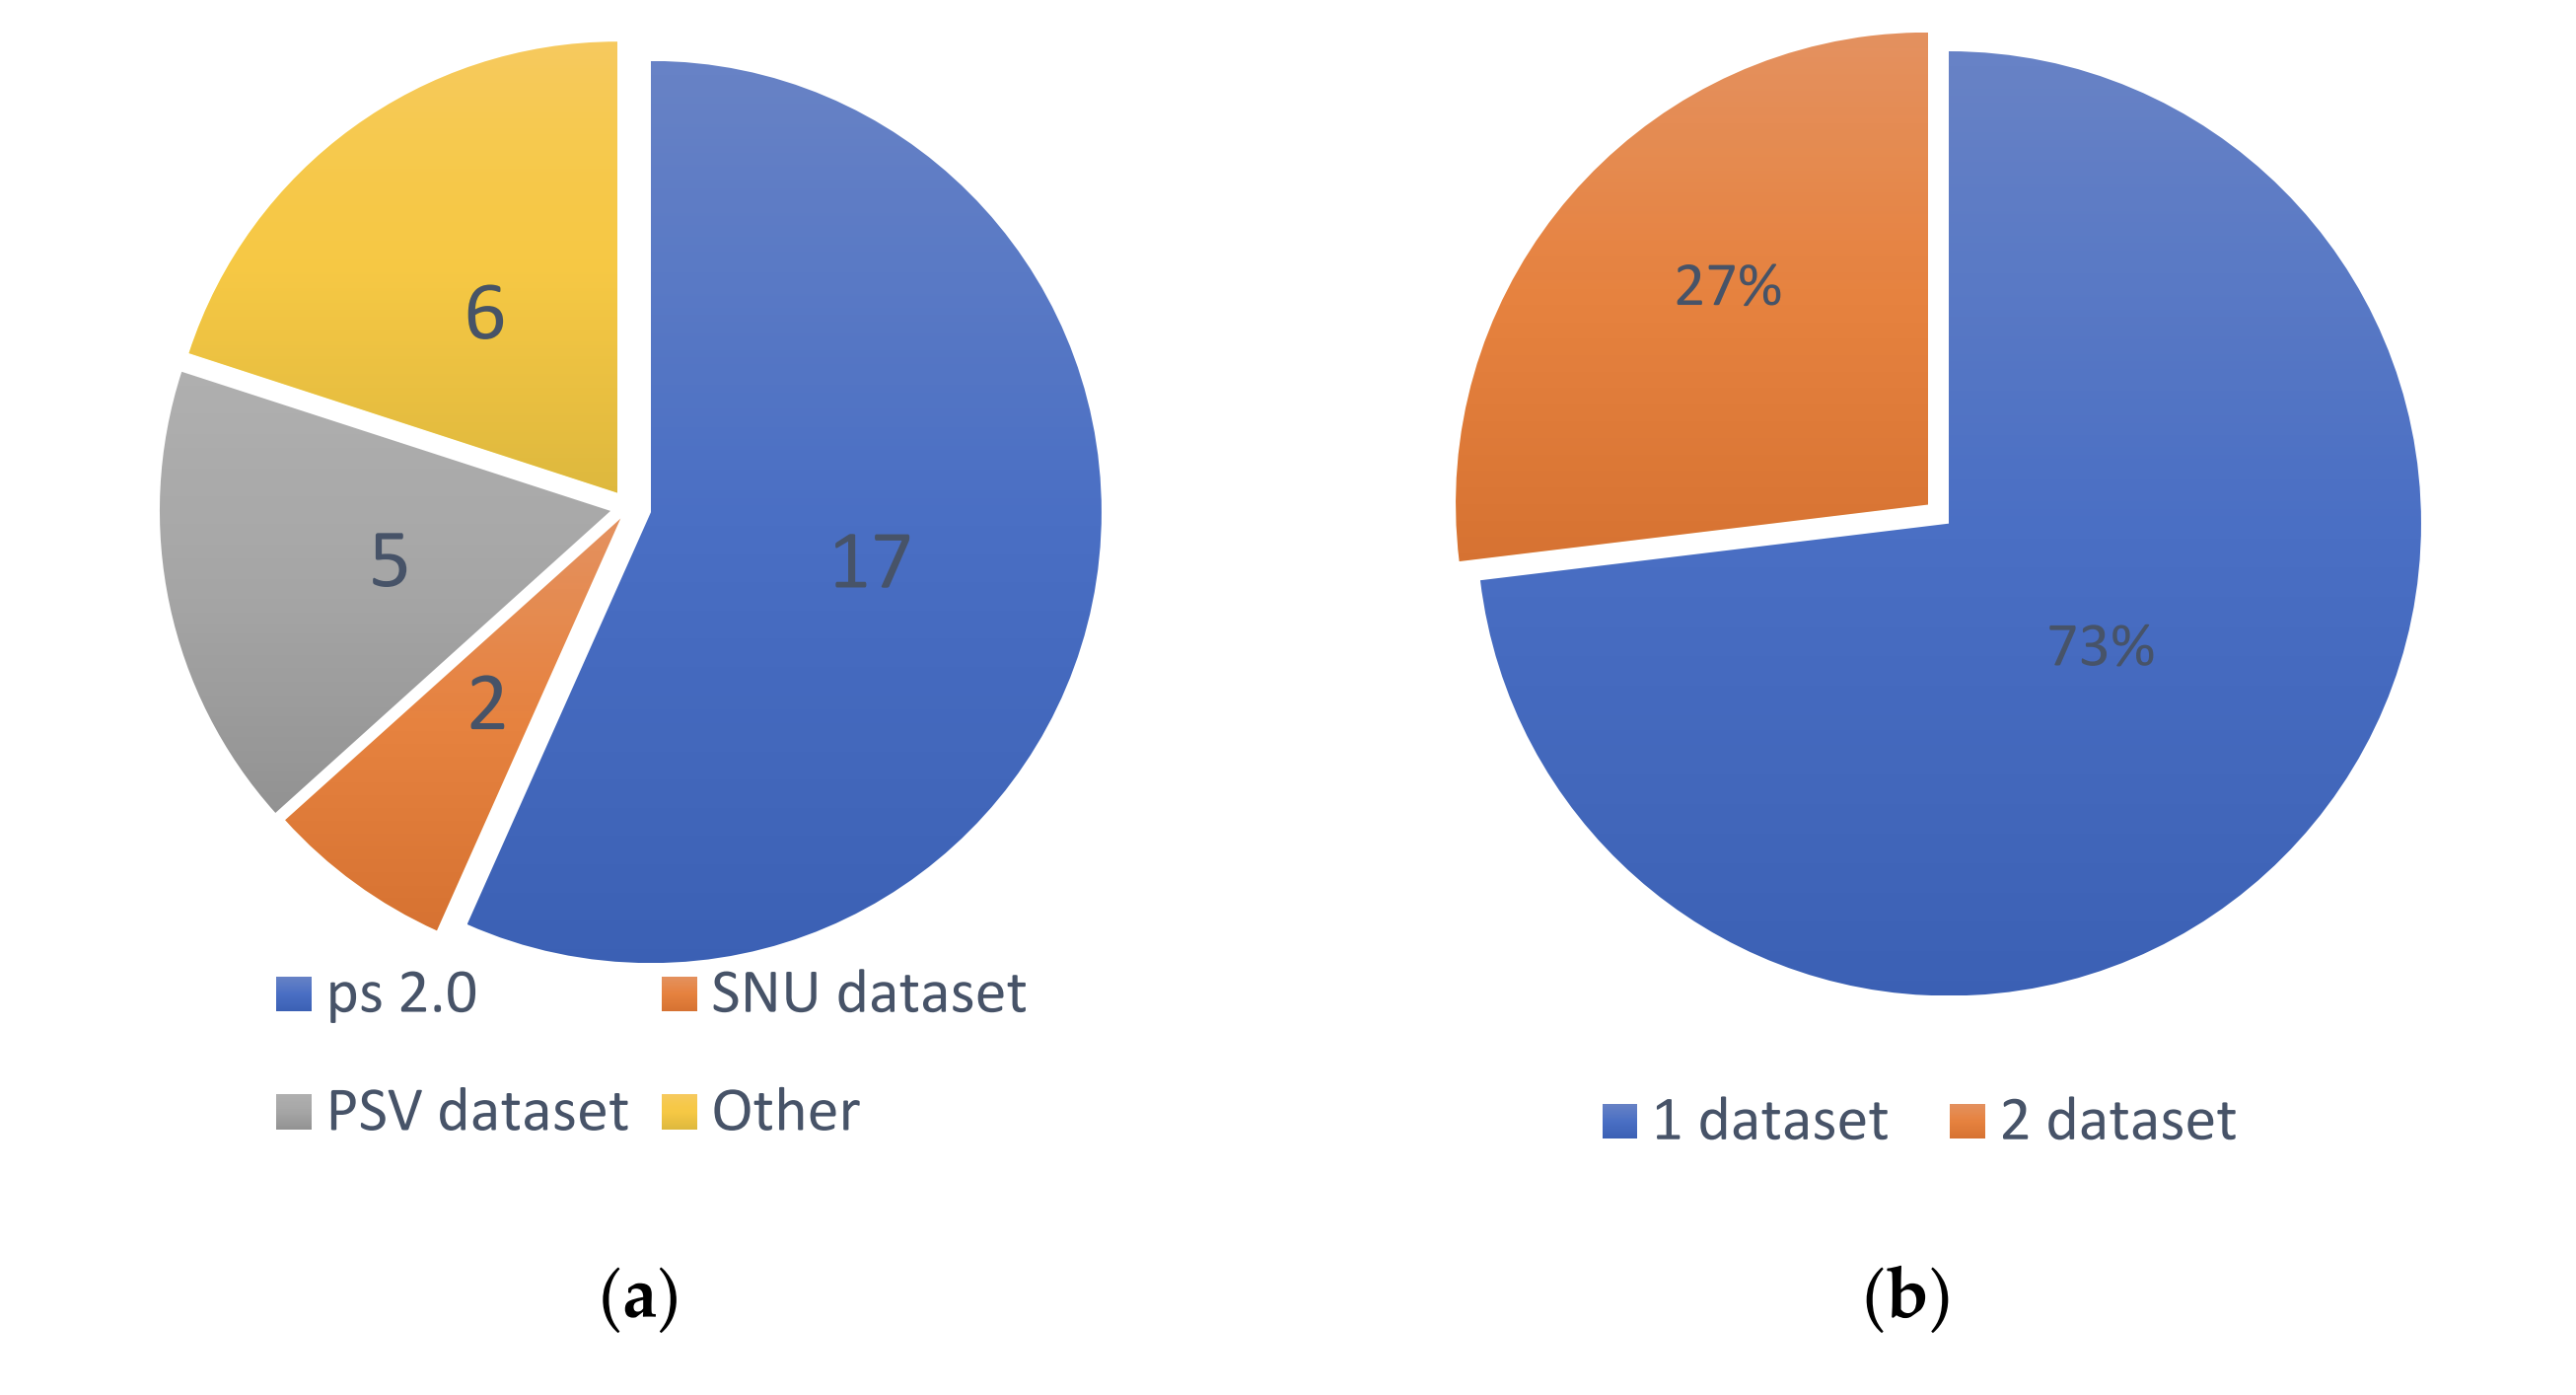
\includegraphics[width=1\linewidth]{figures/chp1/datasets.png}
  \caption{数据集使用分布情况\cite{wong2023review} \\Fig~\ref{fig_dataset}~Dataset Distribution\cite{wong2023review}}
  \label{fig_dataset}
\end{figure}

图\ref{fig_dataset}（a）展示了所综述作品中数据集的使用分布情况。观察可见，大多数研究（共17项）选择利用ps2.0数据集来评估其方法。此外，有6项研究采用了自行采集且未公开的数据集（标注为"其他"）。而2020年发布的SNU数据集在方法评估中的使用相对有限（仅2项研究）。

图\ref{fig_dataset}（b）描绘了关于所使用数据集数量的评估策略。多数研究（73\%）依赖单一数据集来评估其算法。然而，有27\%的研究在评估中采用了两个数据集，包括将一个公开数据集与另一个自标注数据集相结合，或是同时利用两个公开数据集。采用多个数据集进行评估代表了一种更有前景的研究方向，因为它能够验证方法在不同数据集之间的泛化能力。


\section{停车位检测一般方法}

如图\ref{fig_pip1}所示，停车位检测的典型流程包括以下几个关键环节：首先，输入图像通常是由全景环视系统（AVM）生成的环视图，或是由鱼眼摄像头直接捕捉的鱼眼图像。在送入特征提取骨干网络之前，输入图像需经过预处理步骤，如尺寸调整（Resizing）以及翻转、添加噪声等数据增强技术，以提升模型的鲁棒性。

特征提取模块在停车位检测中起着核心作用，负责提取从低级到高级的特征表示。低级特征包括角点或颜色信息，用于捕捉停车位的局部细节；高级特征则代表更抽象的语义信息，如停车位的整体形状、尺寸及排列布局。

提取出的特征随后被传递至检测、分类或分割模块以生成预测结果。输出预测可以采取多种形式，例如标线点坐标、停车位区域边界，或是代表车位边界的分割掩码。为了优化预测输出，系统通常会利用预定义的几何规则或模板匹配技术进行后处理，确保预测结果符合停车位的预期几何特征。


\begin{figure}[!h] % use float package if you want it here
%\setlength{\abovecaptionskip}{-0.2cm} %调整图片caption与正文之间的间距，table同理。可自己调整。
  \centering
  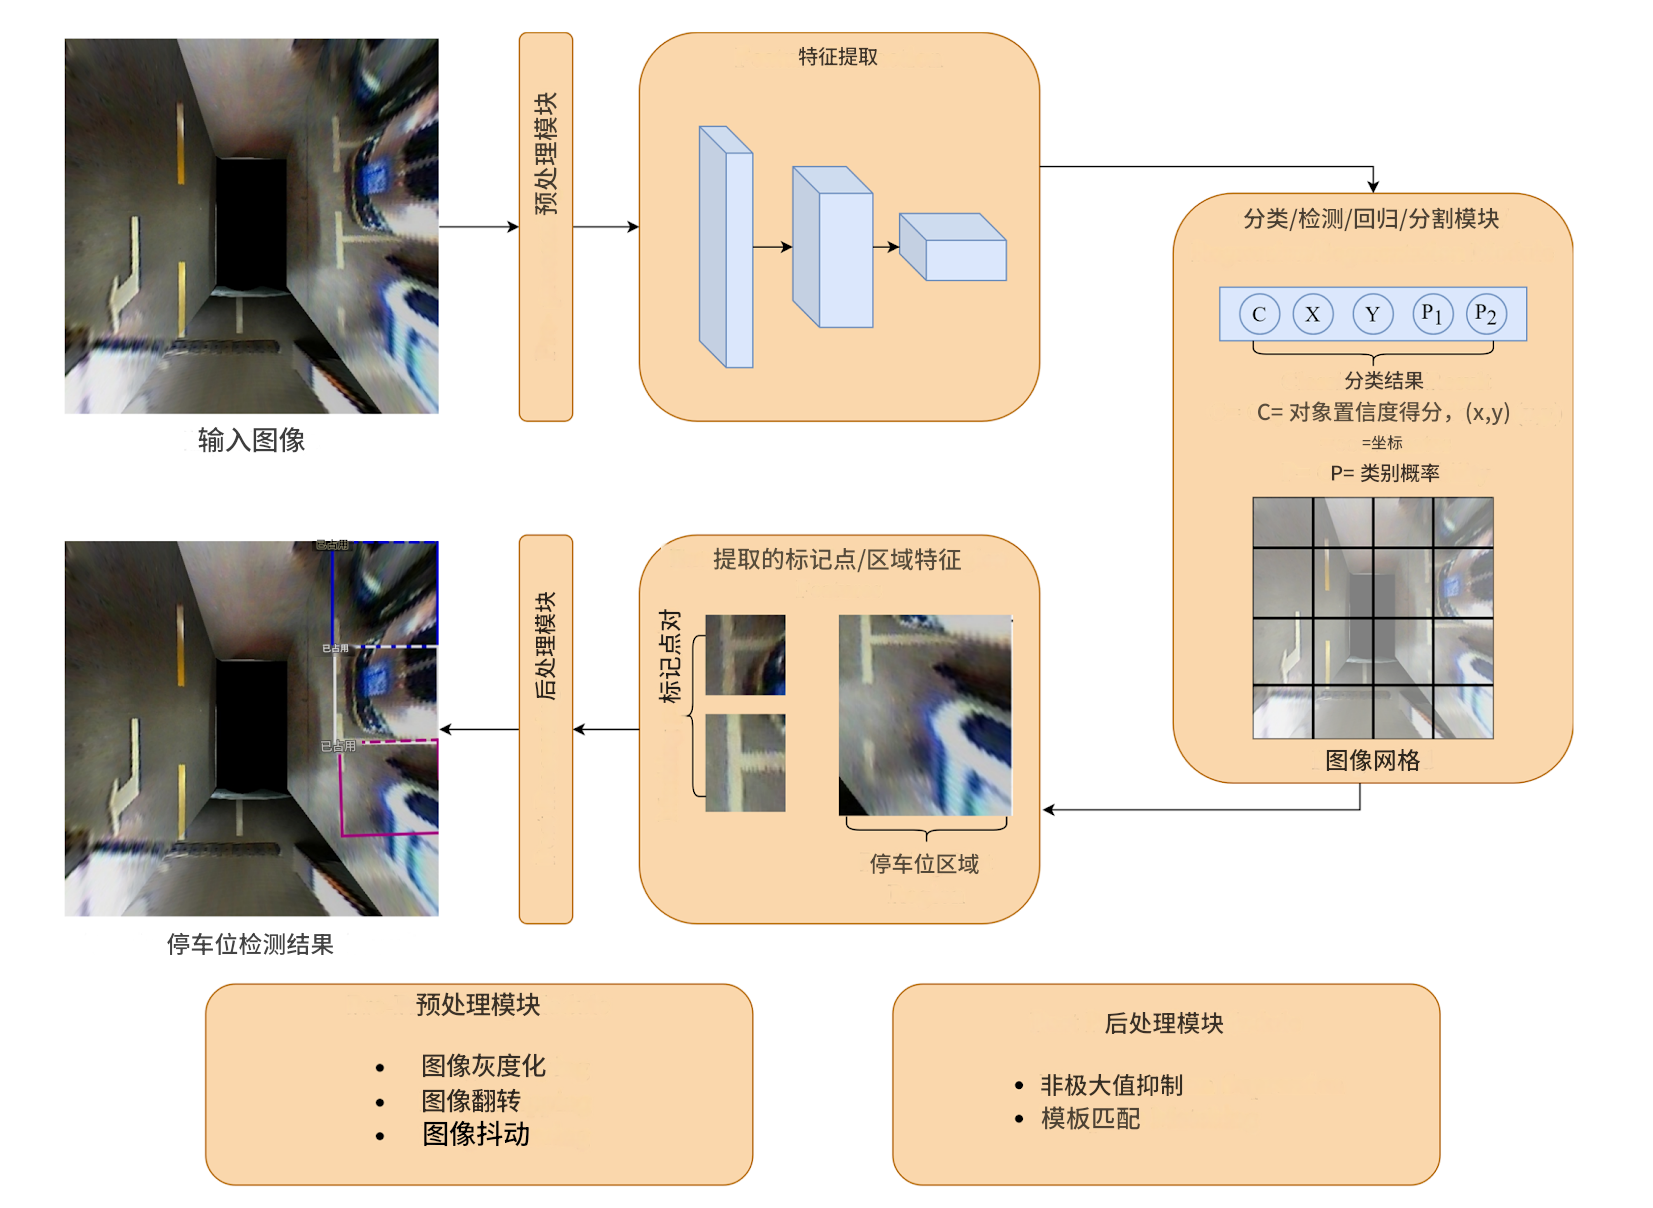
\includegraphics[width=1\linewidth]{figures/chp1/pipline.png}
  \caption{停车位检测的一般流程\cite{wong2023review} \\Fig~\ref{fig_pip1}~General Flow for Parking Slot Detection\cite{wong2023review}}
  \label{fig_pip1}
\end{figure}


\section{模型评估指标}

在停车位检测研究中，传统评估指标多采用查准率（Precision）和查全率（Recall）。然而，这两个指标对阈值选择较为敏感，可能影响评估结果的可靠性。为提供更全面的评估，本文采用平均精度（Average Precision, AP）作为主要评估指标，具体应用\textit{PASCAL VOC 2010}中的全点插值方法，计算方式如下：

\begin{equation}
AP = \sum \Big((Recall_{j+1}-Recall_{j}) \times Precision_{j+1} \Big)
\end{equation}

其中 $j$ 是满足 $Recall_{j} \neq Recall_{j+1}$ 的索引。

查准率和查全率的计算公式如下：

\begin{equation}
Precision = \frac{TP}{TP + FP}
\end{equation}

\begin{equation}
Recall = \frac{TP}{TP + FN}
\end{equation}

式中，$TP$（True Positives）表示正确检测出的真实目标数量，$FP$（False Positives）表示误报为目标的背景区域数量，$FN$（False Negatives）表示未被检测出的真实目标数量。

为明确TP的判定标准，本文将标记点定义为$P=\{x, y, s, t, \theta_{1}, \theta_{2}\}$，其中$(x, y)$表示标记点位置，$s$表示形状，$t$表示类型，$\theta_{1}, \theta_{2}$表示两个边缘的角度（以度为单位）。设$P^{g}=\{x^{g}, y^{g}, s^{g}, t^{g}, \theta_{1}^{g}, \theta_{2}^{g}\}$为真实标记点（Ground Truth），$P^{d}=\{x^{d}, y^{d}, s^{d}, t^{d}, \theta_{1}^{d}, \theta_{2}^{d}\}$为检测到的标记点。当满足以下条件时，认为$P^{g}$被准确识别，$P^{d}$为TP：

\begin{subequations}
  \begin{align}
  (x^{g}-x^{d})^{2} + (y^{g}-y^{d})^{2} < I^{2} \\
|\theta_{1}^{g} - \theta_{1}^{d}| < B \ or \ 360^{\circ} - |\theta_{1}^{g} - \theta_{1}^{d}| < B \\
|\theta_{2}^{g} - \theta_{2}^{d}| < B \ or \ 360^{\circ} - |\theta_{2}^{g} - \theta_{2}^{d}| < B \\
s^{g} = s^{d} \ and \ t^{g} = t^{d}
  \end{align}
  \end{subequations}
  
如果满足这些条件，可以认为 $P^{g}$ 被准确识别，并且 $P^{d}$ 为TP。

本文将停车位定义为 $S=\{(x_{1}, y_{1}), (x_{2}, y_{2}), \theta_{s}\}$，其中 $(x_{1}, y_{1})$ 和 $(x_{2}, y_{2})$ 是两个标记点的坐标，$\theta_{s}$ 表示入口线的方向。对于一个 GT 停车位 $S_{g}=\{(x_{1}^{g}, y_{1}^{g}), (x_{2}^{g}, y_{2}^{g}), \theta_{s}^{g}\}$，如果检测到的停车位 $S_{d}=\{(x_{1}^{d}, y_{1}^{d}), (x_{2}^{d}, y_{2}^{d}), \theta_{s}^{d}\}$ 满足以下等式，则将其视为TP：
\begin{subequations}
  \begin{align}
  (x_{1}^{g}-x_{1}^{d})^{2} + (y_{1}^{g}-y_{1}^{d})^{2} < I^{2} \\
(x_{2}^{g}-x_{2}^{d})^{2} + (y_{2}^{g}-y_{2}^{d})^{2} < I^{2} \\
|\theta_{s}^{g} - \theta_{s}^{d}| < B \ or \ 360^{\circ} - |\theta_{s}^{g} - \theta_{s}^{d}| < B
  \end{align}
  \end{subequations}

即当停车位的两个标记点均位于真实停车位（GT）的$I$个像素范围内，且$S_{d}$与$S_{g}$的角度差小于$B$时，判定为真阳性。对于$512 \times 512$分辨率的图像，通常设定$I=10$，$B=30$。
% 对于 ps2.0，$I=10$；对于 CRPS-D，$I=8.53$，从 $10 \times \frac{512}{600}$ 调整，以适应较小的图像尺寸 $512 \times 512$。

\section{本章小结}

本章系统梳理了停车位检测领域的核心理论基础，为后续研究提供了坚实支撑。具体内容包括：

首先，详细介绍了ps2.0、PSV、SNU三个主流公开数据集，分析了各数据集的图像特征、标注方式及研究应用情况。其中，ps2.0数据集应用最为广泛，SNU数据集作为新兴替代方案展现出一定潜力，但应用仍相对有限。

其次，阐述了停车位检测的通用流程，涵盖图像输入、预处理、特征提取、检测分割及后处理等关键环节，明确了各模块的功能与作用，为后续方法设计提供了参考框架。

最后，定义了模型评估指标体系，重点介绍了平均精度（AP）的计算方法，并详细界定了标记点和停车位的真阳性判定标准，为后续算法评估提供了统一、客观的基准。

通过本章的理论铺垫，为后续章节的方法设计与实验验证奠定了坚实的基础。